% !TeX root = ../editor.tex
\graphicspath{{Skupina22/img/}}

\title{Vpliv šuma in velikosti kontrolnega vzorca na zaznavanje prisluškovanja v protokolu BB84}
\titlerunning{Zaznavanje prisluškovanja v BB84}
\author{Gašper Harej}
\maketitle

\abstract{

}

\section{Uvod}
\label{g22:sec:uvod}

\subsection{Kvantna distribucija ključev in protokol BB84}
\label{g22:sec:qkd-bb84}

\subsection{Prisluškovanje in vpliv šuma}
\label{g22:sec:prisluskovanje-sum}

\subsection{Sorodne raziskave}
\label{g22:sec:sorodne}

\subsection{Raziskovalno vprašanje in hipoteze H1--H3}
\label{g22:sec:vprasanje-hipoteze}


\section{Metode}
\label{g22:sec:metode}

\subsection{Implementacija BB84 v Qiskit Aer}
\label{g22:sec:orodja}

    Za raziskovanje vpliva šuma in velikosti kontrolnega vzorca na zaznavanje prisluškovanja je bila simulacija protokola BB84 implementirana v programskem jeziku Python s pomočjo knjižnice Qiskit Aer \cite{g22:aer-documentation}. 
    Simulacija temelji na zaporednih prenosih posameznih kvantnih bitov, pri katerih sta priprava stanja in meritev predstavljeni s kvantnim vezjem.

    Za kodiranje posameznega klasičnega bita se uporabljata dve medsebojno nepristranski bazi: računsko bazo \(Z=\{\ket{0},\ket{1}\}\) in diagonalno bazo \(X=\{\ket{+},\ket{-}\}\), kjer velja,
    da meritev stanja, pripravljenega v eni bazi, v drugi bazi z enako verjetnostjo vrne katerega koli od obeh možnih izidov \cite{g22:mina2020scalable, g22:lee2023detection}.
    V simulaciji stanja pripravimo s kvantnima vratoma \(X\) in \(H\). 
    Alice za vsak prenos naključno izbere klasični bit $b \in \{0,1\}$ in bazo $B \in \{Z,X\}$. Kvbit je na začetku pripravljen v stanju $\ket{0}$,
    nato pa z uporabo kvantnih vrat $X$ in $H$ pripravimo eno izmed štirih stanj protokola BB84.
    Vrata $X$ spremenijo stanje $\ket{0}$ v $\ket{1}$, vrata $H$ pa omogočajo pripravo stanj diagonalne baze.
    Postopek priprave posameznih stanj je prikazan v tabeli~\ref{g22:tab:priprava_stanj}.

    \begin{table}[htbp]
        \centering
        \caption{Priprava štirih kvantnih stanj protokola BB84.}
        \label{g22:tab:priprava_stanj}
        \begin{tabular}{cccc}
            \toprule
            Bit $b$ & Baza $B$ & Stanje & Kvantna vrata \\
            \midrule
            0 & $Z$ & $\ket{0}$ & -- \\
            1 & $Z$ & $\ket{1}$ & $X$ \\
            0 & $X$ & $\ket{+}$ & $H$ \\
            1 & $X$ & $\ket{-}$ & $X$, nato $H$ \\
            \bottomrule
        \end{tabular}
    \end{table}

    Po pripravi kvantnega stanja Alice kvbit pošlje Bobu, ki za vsak prejeti kvbit neodvisno in naključno izbere merilno bazo $B_B \in \{Z,X\}$ \cite{g22:mina2020scalable}.
    Če izbere računsko bazo $Z$, takoj izvede meritev. Pri izbiri diagonalne baze $X$ pa pred meritvijo uporabi Hadamardova vrata $H$, s katerimi stanja diagonalne baze preslika v računsko bazo.


    \begin{equation}
        H\ket{+} = \ket{0}, \qquad H\ket{-} = \ket{1}.
        \label{g22:eq:hadamard_meritev}
    \end{equation}

    Tako lahko v obeh primerih izvedemo meritev v računski bazi, pri kateri dobimo klasični izid 0 ali 1. Klasični bit, ki ga pridobimo z meritvijo, Bob nato shrani v seznamu izidov meritev, vključno pa tudi informacijo o izbrani bazi.

    Nato si Alice in Bob izmenjata informacije o izbranih bazah, pri čemer ohranita le tiste bite, pri katerih sta izbrala enako bazo. Bob sicer lahko dobi pravilen rezultat tudi pri meritvi v napačni bazi, vendar se to zgodi zgolj naključno. 
    Ker Bob izbere pravilno bazo le v približno polovici primerov, bo po izmenjavi baz ostalo približno polovica prvotnega števila bitov \cite{g22:mina2020scalable}.


    Qiskit Aer omogoča tudi simulacijo različnih modelov šuma brez uporabe fizičnega kvantnega procesorja, kar omogoča nadzorovano raziskovanje vpliva šuma na zaznavanje prisluškovanja.
    Vsak kvbit simuliramo z ločenim enokubitnim vezjem, ki ga izvedemo z eno meritvijo (\texttt{shots=1}). S tem lahko ponavljamo celoten protokol pri različnih eksperimentalnih pogojih.

\subsection{Model prestrezanja in depolarizacijski šum}
\label{g22:sec:model}

\subsubsection{Napad s prestrezanjem in ponovnim pošiljanjem}
\label{g22:sec:intercept-resend}

    V simulaciji je bil implementiran napad s prestrezanjem in ponovnim pošiljanjem (angl. \textit{intercept-resend}), pri katerem prisluškovalka Eve prestreže posamezni kvbit z verjetnostjo $r$.
    Če ga prestreže, izvede meritev v naključno izbrani bazi in nato pošlje Bobu kvbit, pripravljen v stanju, ki ga je pridobila z meritvijo. V naši simulaciji Eve ne pripravi novega kvbita, temveč se prenos nadaljuje z istim kvbitom v stanju po meritvi.
    Takšna izvedba je v obravnavanem idealnem modelu enakovredna ponovni pripravi in pošiljanju izmerjenega stanja \cite{g22:mina2020scalable,g22:lee2023detection}.

    Ker Eve ne pozna baze, v kateri je Alice pripravila kvbit,
    mora merilno bazo izbrati naključno. Če izbere enako bazo
    kot Alice, njena meritev ne spremeni pripravljenega stanja.
    Če pa izbere drugo bazo, sta oba možna izida meritve enako
    verjetna, kvbit pa po meritvi preide v ustrezno stanje
    Evejine baze. Ker to stanje ni enako prvotnemu, lahko
    Bob pri meritvi dobi drugačen bit od tistega, ki ga je
    poslala Alice.

    
    Pri popolnem prestrezanju Eve izmeri vsak poslani kvbit,
    pri čemer z verjetnostjo $1/2$ izbere drugačno bazo kot
    Alice. Poglejmo primer, ko Alice pripravi kvbit v stanju
    $\ket{0}$, Eve pa ga izmeri v diagonalni bazi $X$.
    Ker sta bazi medsebojno nepristranski, Eve z enako
    verjetnostjo izmeri stanje $\ket{+}$ ali $\ket{-}$.
    Obe stanji lahko v računski bazi zapišemo kot

    \begin{equation}
        \ket{+} = \frac{\ket{0}+\ket{1}}{\sqrt{2}},
        \qquad
        \ket{-} = \frac{\ket{0}-\ket{1}}{\sqrt{2}}.
    \end{equation}

    Če Bob nato izbere enako bazo kot Alice, torej $Z$,
    izmeri eno od teh dveh stanj. Ker sta absolutni vrednosti
    amplitud obeh baznih stanj enaki, je verjetnost
    posameznega izida enaka kvadratu pripadajoče amplitude.
    Verjetnost, da Bob izmeri napačen bit $1$, je zato
    v obeh primerih

    \begin{equation}
        P(1 \mid \ket{+}) =
        P(1 \mid \ket{-}) =
        \left|\frac{1}{\sqrt{2}}\right|^2
        = \frac{1}{2}.
    \end{equation}

    Pri izračunu QBER upoštevamo le bite, pri katerih sta Alice in Bob izbrala enako bazo, saj se ostali
    pri uskladitvi baz zavržejo. V idealnem kanalu
    napaka tako nastane, kadar Eve izbere napačno bazo
    in Bob posledično izmeri napačen bit.
    Pri popolnem prestrezanju zato pričakovani QBER
    znaša $1/2 \cdot 1/2 = 1/4$, oziroma $25\,\%$
    \cite{g22:mina2020scalable,g22:lee2023detection}.

    Če Eve posamezni kvbit prestreže le z verjetnostjo
    $r$, se pričakovani QBER v idealnem kanalu zmanjša na

    \begin{equation}
        q_{\mathrm{Eve}} = \frac{r}{4}.
        \label{g22:eq:qber_eve}
    \end{equation}

\subsubsection{Depolarizacijski model šuma}
\label{g22:sec:depolarizacija}

    Da bi Alice in Bob preverila prisotnost morebitnega prisluškovanja, javno primerjata vrednosti naključno izbranega dela ohranjenih bitov. Ker pa lahko napake nastanejo tudi zaradi šuma v kvantnem kanalu, samo neskladje med biti še ne dokazuje prisotnosti Eve \cite{g22:lee2023detection,g22:fiorini2024estimating}.


    Za modeliranje napak pri prenosu kvantnih stanj je bil izbran depolarizacijski šumni kanal.
    Ta omogoča nadzorovano spreminjanje jakosti šuma z enim parametrom, pri čemer enako vpliva na obe bazi protokola BB84.
    Tako lahko raziskujemo vpliv šuma na zaznavanje prisluškovanja, ne da bi bili rezultati odvisni od izbire merilne baze \cite{g22:aer-depolarizing}.


    Depolarizacijski kanal z večanjem jakosti šuma približuje začetno kvantno stanje maksimalno mešanemu stanju, pri katerem sta oba možna rezultata meritve enako verjetna, ne glede na izbrano merilno bazo.
    Matematično ga opišemo z izrazom

    \begin{equation}
        \mathcal{D}_{\lambda}(\rho)
        = (1-\lambda)\rho+\lambda\frac{I}{2},
        \label{g22:eq:depolarizing}
    \end{equation}

    kjer je $\rho$ gostotna matrika stanja kvbita pred delovanjem šuma, $I$ identitetna matrika, $\lambda$ pa parameter depolarizacije \cite{g22:aer-documentation}.

    Za primer vzemimo kvbit, pripravljen v stanju $\ket{0}$, ki ga lahko predstavimo z gostotno matriko
    $\rho=\ket{0}\bra{0}=
    \bigl(\begin{smallmatrix}
    1&0\\0&0
    \end{smallmatrix}\bigr)$.
    Maksimalno mešano stanje pa je
    $I/2=\bigl(\begin{smallmatrix}
    1/2&0\\0&1/2
    \end{smallmatrix}\bigr)$.

    Pri $\lambda=0$ kanal ohrani prvotno stanje, pri $\lambda=1$ pa dobimo maksimalno mešano stanje, pri katerem sta oba rezultata meritve enako verjetna.

    V simulaciji je bil šumni model vezan na identitetno operacijo \texttt{id}, vstavljeno po morebitnem prestrezanju Eve in pred Bobovo meritvijo.
    Ker se je ta operacija v posameznem vezju pojavila samo enkrat, je bil vsak kvbit izpostavljen enemu depolarizacijskemu kanalu.
    Takšna postavitev je omogočala, da smo v obeh scenarijih, z Eve in brez nje, uporabili enake pogoje šuma.
    Pri tem smo pripravo stanj in meritve obravnavali kot idealne, šum pa je predstavljal motnje med prenosom kvbita.

\subsubsection{Pričakovani delež bitnih napak}
\label{g22:sec:pricakovani-qber}


    Iz opisanega modela lahko izpeljemo pričakovani
    delež bitnih napak tudi brez prisotnosti Eve.
    Poglejmo primer, ko Alice pripravi kvbit v stanju
    $\ket{0}$, Bob pa ga izmeri v računski bazi $Z$.
    Brez šuma bi Bob vedno dobil pravilen rezultat $0$.
    Po delovanju depolarizacijskega kanala pa stanje
    opišemo z matriko

    \begin{equation}
        \mathcal{D}_{\lambda}(\ket{0}\bra{0})
        =
        \begin{pmatrix}
            1-\lambda/2 & 0 \\
            0 & \lambda/2
        \end{pmatrix}.
    \end{equation}

    Diagonalna elementa matrike predstavljata
    verjetnosti rezultatov meritve v računski bazi.
    Verjetnost, da Bob namesto poslanega bita $0$
    izmeri napačen bit $1$, je torej $\lambda/2$.
    Ker depolarizacijski kanal enako vpliva na
    vsa štiri stanja protokola BB84, znaša
    pričakovani QBER brez prisluškovanja

    \begin{equation}
        q_0=\frac{\lambda}{2}.
        \label{g22:eq:qber_no_eve}
    \end{equation}



    Kadar je prisotna tudi Eve, moramo poleg šuma upoštevati
    še napake, ki nastanejo zaradi prestrezanja. Kot smo
    pokazali v enačbi~\eqref{g22:eq:qber_eve}, znaša
    pričakovani delež teh napak v idealnem kanalu $r/4$.

    
    Pri tem ne moremo preprosto sešteti napak zaradi
    prestrezanja in šuma, saj lahko šum spremeni tudi
    stanje kvbita, ki ga je pred tem že zmotila Eve.
    
    Iz enačbe~\eqref{g22:eq:depolarizing} sledi, da
    končno stanje sestavljata dva prispevka.
    Prvi z utežjo $1-\lambda$ ohranja stanje po
    morebitnem prestrezanju, pri katerem je
    verjetnost napačnega bita $r/4$. Drugi z utežjo
    $\lambda$ predstavlja maksimalno mešano stanje,
    pri katerem je verjetnost napačnega bita $1/2$.
    Pričakovani QBER ob prisotnosti Eve je zato
    
    \begin{equation}
        q_1 = (1-\lambda)\frac{r}{4}
            + \lambda\frac{1}{2}.
        \label{g22:eq:qber_with_eve}
    \end{equation}
    




Da bi ugotovili, kako izrazito prisluškovanje vpliva
na delež napak pri različnih jakostih šuma,
primerjamo pričakovani QBER ob prisotnosti Eve
in brez nje. Razlika med njima znaša

\begin{equation}
    q_1-q_0=(1-\lambda)\frac{r}{4}.
    \label{g22:eq:qber_difference}
\end{equation}

Iz izraza je razvidno, da se pri nespremenjenem
deležu prestrezanja z večanjem jakosti šuma
razlika med pričakovanima deležema napak zmanjšuje.
Vpliv prisluškovanja je zato v bolj šumnem kanalu
manj izrazit, kar lahko oteži njegovo zaznavanje.



\subsection{Kontrolni vzorec in statistični test}
\label{g22:sec:test}


    Po uskladitvi baz Alice in Bob izmed ohranjenih bitov
    naključno izbereta $m$ bitov, ki sestavljajo kontrolni
    vzorec \cite{g22:fiorini2024estimating}.
    Na izbranih mestih primerjata vrednosti svojih
    bitov in preštejeta število neskladij $k$.
    Opaženi delež bitnih napak v kontrolnem vzorcu
    tako znaša \cite{g22:lee2023detection}

    \begin{equation}
        \hat{q}=\frac{k}{m}.
        \label{g22:eq:observed-qber}
    \end{equation}


%verjetno bo ta del treba malo skrajšati%
Ker so kvantne meritve naključne, se lahko opaženi
delež napak $\hat{q}$ razlikuje od pričakovanega
deleža $q_0$, tudi kadar Eve ni prisotna.
Zato samo višji opaženi QBER še ne dokazuje
prisluškovanja.

Za statistično obravnavo napak posamezni kontrolni
bit predstavimo z Bernoullijevo slučajno spremenljivko
$X_i$, ki jo definiramo kot

\begin{equation}
    X_i =
    \begin{cases}
        1, & \text{če se Aličin in Bobov bit razlikujeta},\\
        0, & \text{če se bita ujemata}.
    \end{cases}
\end{equation}

Če Eve ni prisotna, je verjetnost napake pri
posameznem bitu enaka $P(X_i=1)=q_0$, kot smo
izpeljali v enačbi~\eqref{g22:eq:qber_no_eve}
\cite{g22:lee2023detection}.

Binomska porazdelitev opisuje število določenih
dogodkov pri več neodvisnih ponovitvah, kadar
ima dogodek pri vsaki ponovitvi enako verjetnost.
Ker v naši simulaciji predpostavljamo neodvisne
prenose kvbitov in enako verjetnost napake
$q_0$ pri vseh kontrolnih bitih, lahko skupno
število napak v vzorcu velikosti $m$
opišemo z binomsko porazdelitvijo
\cite{g22:scipy-binomial}:

\begin{equation}
    K = \sum_{i=1}^{m} X_i
    \sim \operatorname{Bin}(m,q_0).
    \label{g22:eq:binomial-model}
\end{equation}
%%


Na podlagi binomske porazdelitve lahko preverimo, ali je
opaženo število napak $k$ še skladno s pričakovanim šumom.
Pri tem predpostavimo, da Eve ni prisotna, kar označimo
z ničelno hipotezo $H_0$. Zanima nas, kolikšna je
verjetnost, da bi ob tej predpostavki dobili vsaj
$k$ napak. To verjetnost, imenovano p-vrednost,
izračunamo z izrazom

\begin{equation}
    p = P(K \geq k \mid H_0)
      = \sum_{j=k}^{m}
        \binom{m}{j}q_0^j(1-q_0)^{m-j}.
    \label{g22:eq:p-value}
\end{equation}

Za izračun p-vrednosti smo uporabili funkcijo
\texttt{binomtest} iz knjižnice SciPy, ki izvede
eksaktni binomski test. Ta verjetnost izračuna
neposredno iz binomske porazdelitve, zato
približek z normalno porazdelitvijo ni potreben.
To je posebej uporabno pri manjših kontrolnih
vzorcih, ki jih prav tako obravnavamo v raziskavi
\cite{g22:scipy-binomtest}.

Kot mejo za zaznavanje prisluškovanja smo izbrali
stopnjo značilnosti $\alpha=0{,}05$. Če je izračunana
p-vrednost manjša ali enaka tej meji, zavrnemo
predpostavko, da so napake posledica samo šuma,
in sprožimo alarm za prisluškovanje. S takšno
izbiro omejimo teoretično verjetnost lažnega
alarma na največ $5\,\%$, kadar Eve ni prisotna
in veljajo predpostavke našega modela.



\subsection{Parametri eksperimentov in uporabljene metrike}
\label{g22:sec:poskusi}
\label{g22:sec:metrike}

    
    
    V eksperimentih smo preverjali, kako stopnja šuma
    in velikost kontrolnega vzorca vplivata na
    uspešnost zaznavanja prisluškovanja.
    V posamezni simulaciji je Alice poslala
    $N=2400$ kvbitov.

    Za parameter depolarizacijskega šuma smo izbrali
    vrednosti
    $\lambda \in \{0{,}06;\ 0{,}10;\ 0{,}20;\
    0{,}40;\ 0{,}50\}$.
    S tem smo zajeli različne stopnje šuma, pri
    katerih pričakovani QBER brez Eve znaša od
    $3\,\%$ do $25\,\%$. Tako lahko preverimo,
    kako povečevanje šuma vpliva na zaznavanje
    prisluškovanja.

    Delež prestreženih kvbitov smo spreminjali med
    $r \in \{0;\ 0{,}10;\ 0{,}20;\ 0{,}50;\ 1\}$.
    Vrednost $r=0$ predstavlja prenos brez Eve,
    $r=1$ pa prestrezanje vseh kvbitov.
    Vmesne vrednosti nam omogočajo preverjanje
    zaznavanja pri delnem prestrezanju.

    Za vsako kombinacijo parametrov smo preverili
    kontrolne vzorce velikosti
    $m \in \{20; 50; 100; 300; 500; 1000\}$.
    Izbrali smo tako majhne kot večje vzorce,
    da bi ugotovili, kako število preverjenih
    bitov vpliva na uspešnost zaznavanja.

%%
Za vsako kombinacijo šuma in deleža prestrezanja
smo simulacijo neodvisno ponovili 2000-krat.
Pri vsaki ponovitvi smo na novo naključno
izbrali bite in baze ter simulirali prenos
in meritve kvbitov.

Po uskladitvi baz smo naključno izbrali
1000 različnih ohranjenih bitov. Iz tega
izbora smo sestavili kontrolne vzorce vseh
šestih velikosti, tako da so bili manjši
vzorci vključeni v večje. S tem smo lahko
primerjali vpliv velikosti vzorca pri istem
prenosu kvbitov, ne da bi na primerjavo
vplivale razlike med posameznimi prenosi.
Za vsako velikost vzorca smo posebej izvedli
statistični test in zabeležili, ali je bil
sprožen alarm za prisluškovanje.
 %%


    

Uspešnost zaznavanja prisluškovanja smo ocenili
z metrikama TPR (\textit{True Positive Rate})
in FPR (\textit{False Positive Rate}).
Tudi \citet{g22:lee2023detection} za ocenjevanje
zaznavanja prisluškovanja uporabljajo metriki
FPR in FNR (\textit{False Negative Rate}).
Namesto FNR smo uporabili TPR, saj nas zanima
predvsem delež uspešno zaznanih primerov
prisluškovanja. Metriki sta povezani z
$\mathrm{TPR}=1-\mathrm{FNR}$.


TPR predstavlja delež simulacij, v katerih
je test pravilno zaznal prisluškovanje,
ko je bila Eve prisotna ($r>0$).
Izračunali smo ga kot

\begin{equation}
    \mathrm{TPR} =
    \frac{\text{število zaznav prisluškovanja v 2000 ponovitvah pri } r>0}{2000}.
    \label{g22:eq:tpr}
\end{equation}

FPR predstavlja delež simulacij, v katerih
je test napačno zaznal prisluškovanje,
čeprav Eve ni bila prisotna ($r=0$):

\begin{equation}
    \mathrm{FPR} =
    \frac{\text{število zaznav prisluškovanja pri } r=0}{2000}.
    \label{g22:eq:fpr}
\end{equation}

TPR smo izračunali posebej za vsako kombinacijo
šuma, deleža prestrezanja in velikosti kontrolnega
vzorca, FPR pa za vsako stopnjo šuma in velikost
vzorca pri $r=0$. Cilj je doseči čim višji TPR
ob čim nižjem FPR.


    Ker smo TPR in FPR izračunali na podlagi
    2000 ponovitev, se lahko izmerjene vrednosti
    zaradi naključnosti nekoliko razlikujejo od
    dejanskih verjetnosti. Zato smo izračunali
    tudi 95-\% intervale zaupanja po Wilsonovi metodi,
    s katerimi ocenimo negotovost naših rezultatov.
    Wilsonovo metodo smo izbrali, ker je primerna
    tudi za deleže blizu $0\,\%$ ali $100\,\%$.
    Za izračun smo uporabili knjižnico SciPy
    \cite{g22:scipy-binomtest}.


Za primerjavo z rezultati simulacij smo iz
binomske porazdelitve izračunali tudi teoretične
vrednosti TPR in FPR. Tako smo lahko preverili,
kako dobro se rezultati simulacij ujemajo
s pričakovanji našega statističnega modela.





\section{Rezultati}
\label{g22:sec:rezultati}

\subsection{Vpliv velikosti kontrolnega vzorca}
\label{g22:sec:rezultati-h1}

Najprej smo preverili, kako velikost kontrolnega
vzorca vpliva na uspešnost zaznavanja
prisluškovanja. Na sliki~\ref{g22:fig:h1}
je prikazan TPR pri različnih velikostih
kontrolnega vzorca in stopnjah šuma.
Delež prestreženih kvbitov je bil pri
vseh prikazanih rezultatih $r=0{,}20$.

\begin{figure}[htbp]
    \centering
    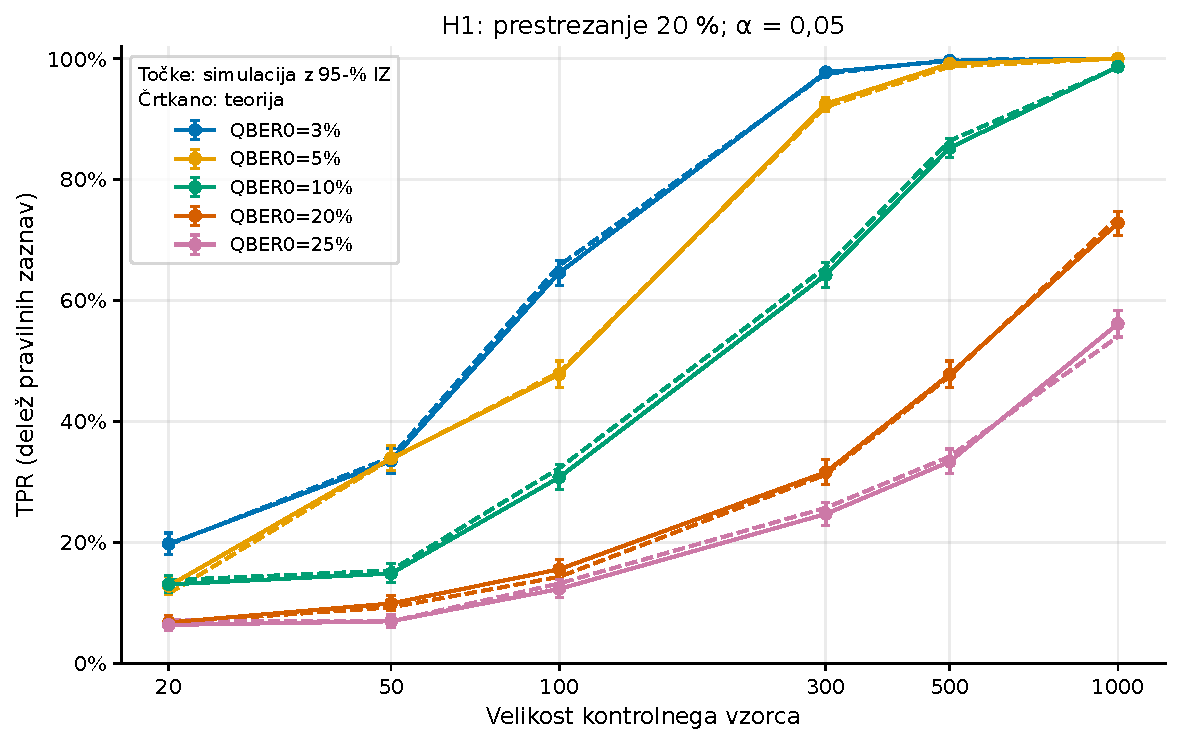
\includegraphics[width=0.8 \linewidth]
        {Skupina22/img/h1_tpr_vs_sample.pdf}
    \caption{Vpliv velikosti kontrolnega vzorca
    na delež pravilnih zaznav pri
    $20\,\%$ prestrezanju. Točke prikazujejo
    rezultate simulacij s 95-\% intervali
    zaupanja, črtkane črte pa teoretične
    napovedi.}
    \label{g22:fig:h1}
\end{figure}

Rezultati kažejo, da se z večanjem kontrolnega
vzorca povečuje tudi uspešnost zaznavanja
prisluškovanja. Pri osnovnem QBER $3\,\%$
se je TPR povečal z $19{,}75\,\%$ pri
vzorcu 20 bitov na $100\,\%$ pri 1000 bitih.
Pri osnovnem QBER $25\,\%$ pa se je
v enakem razponu povečal le s
$6{,}35\,\%$ na $56{,}15\,\%$.

Iz rezultatov je razvidno, da večji
kontrolni vzorci omogočajo uspešnejše
zaznavanje, vendar je pri višjih stopnjah
šuma izboljšanje precej počasnejše.
Izmerjene vrednosti se dobro ujemajo
s teoretičnimi napovedmi.



\subsection{Vpliv šuma}
\label{g22:sec:rezultati-h2}

Na sliki~\ref{g22:fig:h2} je prikazan vpliv
šuma na uspešnost zaznavanja prisluškovanja
pri različnih deležih prestrezanja.
Velikost kontrolnega vzorca je bila pri
vseh prikazanih rezultatih $m=300$.

\begin{figure}[htbp]
    \centering
    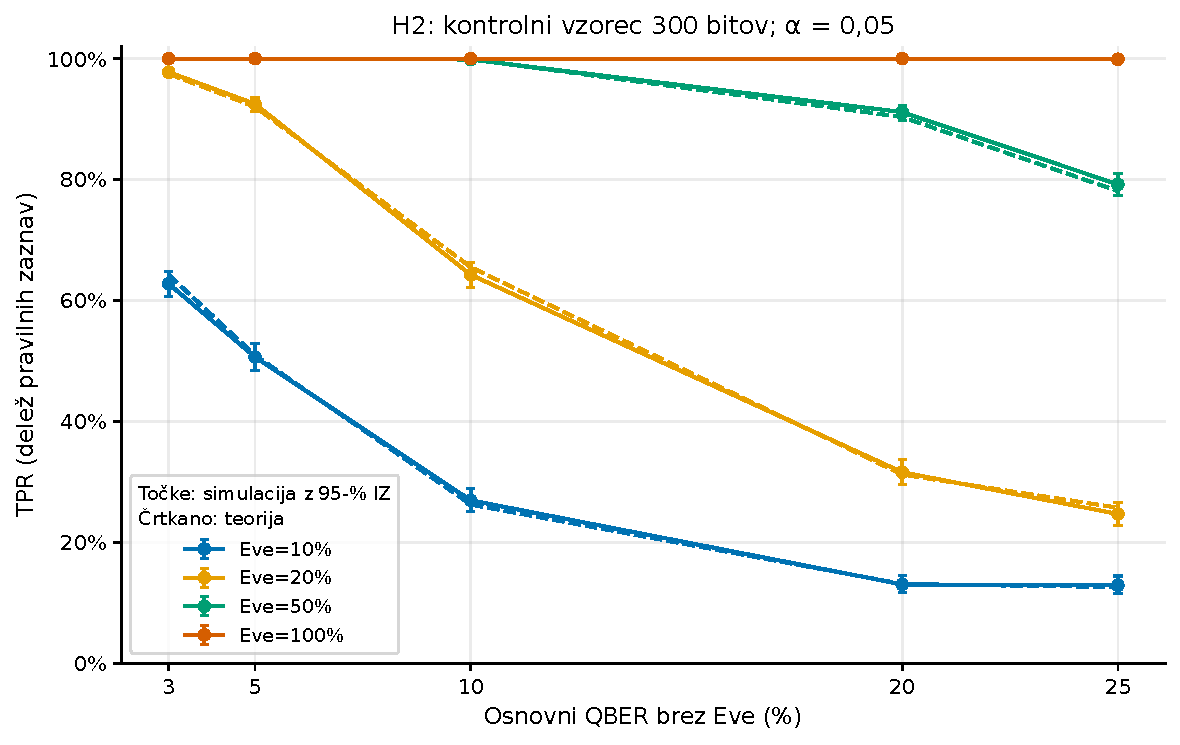
\includegraphics[width=\linewidth]
        {Skupina22/img/h2_tpr_vs_noise.pdf}
    \caption{Vpliv osnovnega QBER na delež
    pravilnih zaznav pri kontrolnem vzorcu
    velikosti 300 bitov. Točke prikazujejo
    rezultate simulacij s 95-\% intervali
    zaupanja, črtkane črte pa teoretične
    napovedi.}
    \label{g22:fig:h2}
\end{figure}

Rezultati kažejo, da se z večanjem šuma
uspešnost zaznavanja prisluškovanja zmanjšuje.
Pri $20\,\%$ prestrezanju se je TPR zmanjšal
s $97{,}75\,\%$ pri osnovnem QBER $3\,\%$
na $24{,}70\,\%$ pri osnovnem QBER $25\,\%$.

Vpliv šuma je izrazitejši pri manjših deležih
prestrezanja. Pri $100\,\%$ prestrezanju pa
je test prisluškovanje zaznal v skoraj vseh
simulacijah tudi pri najvišji stopnji šuma.
Podobno kot pri prejšnjem eksperimentu se
izmerjene vrednosti dobro ujemajo s
teoretičnimi napovedmi.


\subsection{Lažne zaznave prisluškovanja}
\label{g22:sec:rezultati-fpr}

Preverili smo tudi pogostost lažnih zaznav
prisluškovanja, kadar Eve ni bila prisotna
($r=0$). Pri vseh 30 kombinacijah šuma in
velikosti kontrolnega vzorca je bil izmerjeni
FPR med $1{,}4\,\%$ in $4{,}75\,\%$.

Nobena izmerjena vrednost ni presegla izbrane
meje $5\,\%$, kar je skladno s pričakovanim
delovanjem statističnega testa. Izmerjene
vrednosti se zaradi naključnosti simulacij
nekoliko razlikujejo od teoretičnih napovedi.



\section{Razprava}
\label{g22:sec:razprava}

\subsection{Interpretacija in primerjava z literaturo}
\label{g22:sec:interpretacija}

\subsection{Omejitve modela}
\label{g22:sec:omejitve}

\subsection{Kaj ni delovalo}
\label{g22:sec:neuspehi}


\section{Zaključek}
\label{g22:sec:zakljucek}


\section*{Doprinosi avtorjev}



\section*{Izjava o uporabi generativne umetne inteligence}
Pri pripravi seminarske naloge sem uporabljal generativno umetno inteligenco (ChatGPT) kot pomoč pri razumevanju protokola BB84 in statističnih metod, načrtovanju eksperimentov, razlagi in pregledu programske kode ter iskanju in preverjanju literature. Uporabljal sem jo tudi za pomoč pri oblikovanju posameznih odstavkov, izboljšanju razumljivosti besedila in zapisu matematičnih izrazov v LaTeXu.

Predloge sem pregledal in prilagodil ter jih vključil po lastni presoji. Za pravilnost končne vsebine, implementacije, rezultatov in zaključkov odgovarjam sam.